\title{Human Perception of the Light}
\author{Vicente González Ruiz}
\maketitle

\section{Physics}
The light produces an excitation of the photo-sensitive cells of our
retina (cones and rods) that transmit nerve impulses to our brain.

\section{Intensity sensitivity~\cite{gonzalez1992digital}}
The level of perceived (subjective) illumination is, in general, a
logarithmic function of the intensity of light incident on the eye
(Weber-Fechner's Law). Moreover, The perceptibility of luminance
changes varies inversely with the mean luminance
level~\cite{taubman2012jpeg2000}. See
  Fig.~\ref{fig:light_perception_threshold}.

\begin{figure}
  %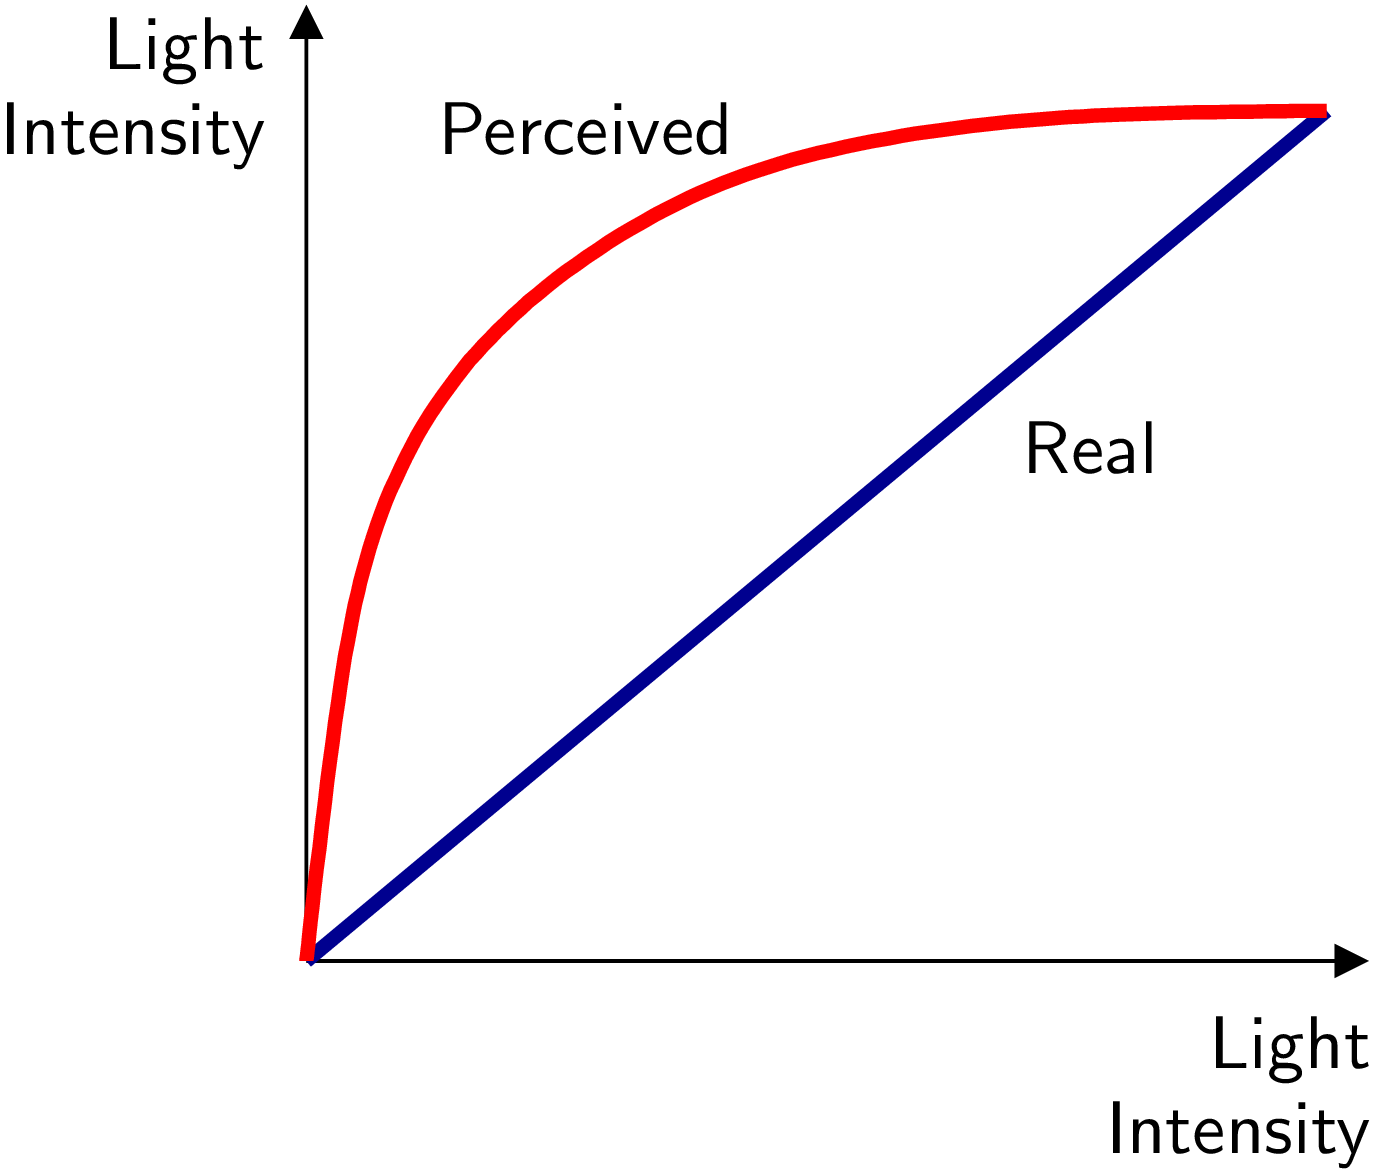
\includegraphics[width=12cm]{umbral_de_vision}%{6cm}{600} %
  \svg{umbral_de_vision}{600}
  \caption{Perception threshold of the light intensity.} %
  \label{fig:light_perception_threshold}
\end{figure}

However, the perceived luminous intensity (or luminance) also depends on many other factors:
\begin{enumerate}
\tightlist
\item The state of previous adaptation of the eye.
\item The observation time.
\item The area of the retina impressed.
\item The luminance of the contour.
\item The color.
\end{enumerate}

\section{Contrast sensitivity}
Humans are more sensible to variations of the low frequencies in
images than to variations of the high frequencies. See the
\href{CSF.html}{Campbell and Robson CSF test chart}.
  
\section{The perceived luminance depends on the observation time}

See Fig~\ref{fig:perceived_luminance_along_time}.

\begin{figure}
  \png{punto_y_difuminado}%{6cm}{600} %
  \caption{Perceived luminance along time. Fixing the eyes on the black point, the gray outline should disappear.} %
  \label{fig:perceived_luminance_along_time}
\end{figure}

\section{The perceived luminance depends on the area of the retina impressed}
To verify that the perceived level of illumination depends on the area
of the retina impressed, perform the following experiment:

Enter a darkened room (with a very low level of illumination) from another room in which there is enough light, and try to discern an object by looking directly at it and looking at it out of the corner of your eye. You will see that the second option is better because we excite the canes. You will notice, however, that you are not able to distinguish the details of the object.

This is also shown in the following image (when looking at the white circles, we will see that only when we look at them they look white, others look black). See Fig~\ref{fig:perceived_luminance_vs_angle}.

\begin{figure}
  \png{rectangulos_negros}%{8cm}{800} %
  \caption{Perceived luminance depending on the vision angle.} %
  \label{fig:perceived_luminance_vs_angle}
\end{figure}

\section{The perceived luminance depends on the level of illumination of the contour}

The level of perceived luminance does not depend only on the intensity at a point, but also depends on the intensity of the neighboring points. See Fig~\ref{fig:simultaneous_contrast}.

\begin{figure}
  \png{escaleras1}%{8cm}{800} %
  \png{contraste_simultaneo}%{8cm}{800} %
  \caption{Simultaneous contrast. The intensity of the internal square always have the same intensity.} %
  \label{fig:simultaneous_contrast}
\end{figure}

The HVS tends to overestimate the boundaries between objects.

\section{The perceived luminance depends on the color of the light}
The HVS is more sensitive to yellow and green than blue or red (these are less dazzling). See Fig~\ref{fig:color_perception}.

\begin{figure}
  \png{espectro_visible}%{8cm}{800} %
  \caption{Color perception. All colors appear exactly with the same intensity} %
  \label{fig:color_perception}
\end{figure}

Relative sensibility to the color (see Fig.~\ref{fig:color_relative_sensibility}) causes, for example, that when we spend enough time in a room with only red light or wear red glasses, the threshold of vision is very low (almost the same as we would have achieved if we stayed a long time in the dark).

\begin{figure}
  \png{sensibilidad_relativa}%{8cm}{800} %
  \caption{Relative sensitivity of the HVS depending on the color.} %
  \label{fig:color_relative_sensibility}
\end{figure}

\section{Visual acuity}

Visual acuity measures the ability to discern high frequencies (for example, 2 very close points). It depends primarily on the concentration of cones on the retinal surface and the accuracy of the eye's focus.

The field of vision (area where visual acuity is greater) of the human eye is rectangular ($30^o$ in vertical and $40^o$ in horizontal). Outside of this field, the image does not affect the fovea and is blurred. For this reason, in photographs, in movies, on television, etc., the images are wider than high.

\section{Visual persistence}

If we visualize a static image (frame) during a time interval, it remains "printed" a certain time after the stimulus has disappeared. For this reason, if the frequency of frames is sufficiently high, the disappearance of the previous stimulus can merge with the appearance of the next one. In this way, it may seem that the image is fixed (it does not blink), when in reality it is not like that.

This is used in film and television where 50 (PAL system) or 60 (NTCS system) frames / second are presented respectively. However, even at these frequencies it is possible to see the blinking if the level of luminance of the frames is very high.

\section{Feeling of movement}

Related to visual persistence is the sensation of movement. When the frequency of static images is sufficient (at least 16 frames/second), the SVH interpolates the missing motion between frames and reconstructs the actual scene.

For example, in the vintage cinema 24 FPS are presented, although each frame is repeated once to avoid blinking. PAL TV shows 25 FPS (frames per second) and NTSC TV 30 FPS. In high definition television the number of frames increases up to 50 fps or 60 FPS.

\section{Spatial masking}

The HVV tends to recognize more easily the areas of an image that have simple forms or that form textures, as opposed to others that are not more complex (such as ``noise''). Thanks to this, there are the CAPTCHAs (Completely Automated Public Turing Test to Tell Computers and Hummands Apart), images that hide the information by putting characters on noisy backgrounds. See Fig.~\ref{fig:cpatcha}.

\begin{figure}
  \png{noisy_CAPTCHA}%{4cm}{400} %
  \png{CAPTCHA_theater}%{4cm}{400} %
  \caption{Different captchas.} %
  \label{fig:cpatcha}
\end{figure}

\section{Temporal masking}

The HVS needs a specific time to perceive the appearance of a certain region of an image that did not exist before. For example, in a football match, when we look at the ball or the players, we do not appreciate the texture of the grass that has just appeared in the current image with respect to a previous image, until a certain time elapses.

\section{Other visual effects}

The HVS perceives the distance to the objects depending on the color and the area of the sensitized retina. Here we have some examples (in the Fig.~\ref{fig:depth} the red squares seem to be at a different distance than the blue squares).

\begin{figure}
  \png{cuadrados_rojo_y_azules}%{8cm}{800} %
  \caption{Simulating depth.} %
  \label{fig:depth}
\end{figure}

Moving away or getting closer to the image of the Fig~\ref{fig:rotating}, and looking at the black point, we will appreciate how the outer rings will rotate in the opposite direction. This is because the relative position of the objects that appear in the visual scene depends on the area of the sensitized retina.

\begin{figure}
  \png{rueda}%{8cm}{800} %
  \caption{Perceiving rotation.} %
  \label{fig:rotating}
\end{figure}

The image of the Fig.~\ref{fig:limit} puts the perceptive capacity of the SVH to the limit. It is a very high frequency image in which a pair of patterns are repeated periodically. After looking at it for a while, only the part of the image that falls on the fovea is perceived without oscillation (without apparent movement).

\begin{figure}
  \png{mareo}%{8cm}{800} %
  \caption{Simulating depth.} %
  \label{fig:limit}
\end{figure}

The light that falls on the blind spot is not used in the vision process. See Fig~\ref{fig:bind_spot}.

\begin{figure}
  \png{punto_ciego}%{8cm}{800} %
  \caption{Effect of the bind spot. ith the right eye covered, look at the X and vice versa. If the point does not disappear, get closer or stay away from the image.} %
  \label{fig:bind_spot}
\end{figure}

\section{Visual masking in the space domain}
Similar spatial frequencies can mask each other if they have similar
orientations and are localized in the same area. See Fig~\ref{fig:visual_masking}.
  
\begin{figure}
  \png{visual_masking}%{8cm}{800} %
  \caption{Visual masking between a single artifact and Gaussign
    noise, both produced in the wavelet
    domain.~\cite{taubman2012jpeg2000}}
  \label{fig:visual_masking}
\end{figure}

\section{Visual masking in the time domain}
The movement of a object can mask the movement of a different object
in the same scene, being normally the smaller object the masked one.

\bibliography{signal-processing, video-compression, JPEG2000}
